% TODO: Reformat citation and bibliography style, reformat paragraph spacing

\documentclass[12pt, english, openany]{book}

\usepackage[]{graphicx}
\usepackage[]{color}
\usepackage{alltt}
\usepackage[T1]{fontenc}
\usepackage[utf8]{inputenc}
\setcounter{secnumdepth}{3}
\setcounter{tocdepth}{3}
\setlength{\parskip}{\bigskipamount} % sets paragraph spacing
\setlength{\parindent}{0pt}

\usepackage[top=100pt,bottom=100pt,left=68pt,right=66pt]{geometry}
\geometry{a4paper}

\raggedbottom

\usepackage[english]{babel}

% All page numbers positioned at the bottom of the page
\usepackage{fancyhdr}
\fancyhf{} % clear all header and footers
\fancyfoot[C]{\thepage}
\renewcommand{\headrulewidth}{0pt} % remove the header rule
\pagestyle{fancy}

% Changes the style of chapter headings
\usepackage{titlesec}
\titleformat{\chapter}
   {\normalfont\LARGE\bfseries}{\thechapter.}{1em}{}
% Change distance between chapter header and text
\titlespacing{\chapter}{0pt}{25pt}{2\baselineskip}

% Adds table captions above the table per default
\usepackage{float}
\floatstyle{plaintop}
\restylefloat{table}

% Adds space between caption and table
\usepackage[tableposition=top]{caption}

% Adds hyperlinks to references and ToC
\usepackage{hyperref}
\hypersetup{hidelinks,linkcolor = blue} % Changes the link color and hides the
% hideous red border that usually is created

% If multiple images are to be added, a folder (path) with all the images can
% be added here
\graphicspath{ {figures/} }

% Separates the first part of the report/thesis in Roman numerals
\frontmatter


\begin{document}
\selectlanguage{english}

\begin{titlepage}
	\clearpage\thispagestyle{empty}
	\centering
	\vspace{1.2cm}

	% Titles
	{\large \textbf{Midterm Report} \par}
	\vspace{2.5cm}
	{\Huge \textbf{IPSTERS}} \\
  \vspace{1cm}
  {\Huge IPSentinel Terrestrial Enhanced Recognition System} \\
	\vspace{2.5cm}
	{\large \textbf{João Fonseca} \par}
	\vspace{.75cm}
	{\large \textbf{Advisor:} Prof. Fernando Lucas Bação \par}

	\vspace{1.5cm}
    
\includegraphics[scale=0.2]{ims_logo.png}
  \vspace{1.3cm}

	{\normalsize NOVA Information Management School \\
		Instituto Superior de Estatística e Gestão de Informação \\
		Universidade Nova de Lisboa \par}

  \vspace{1.5cm}

	% Set the date
	{\normalsize \textbf \today \par}
	\pagebreak
\end{titlepage}

\chapter*{Abstract}

This report documents the work developed towards the research project "IPSTERS
- IPSentinel Terrestrial Enhanced Recognition System". It focuses on the
exploration of several machine learning (ML) techniques, covering different
stages of a Land Use/Land Cover Classification (LULC) pipeline. These
techniques aim to minimise problems typically found in this kind of data,
namely data ingestion, feature selection, data filtering and classification.



\tableofcontents{}

\clearpage

\listoffigures

\clearpage

\listoftables

\mainmatter

\chapter{Introduction}

The Copernicus programme is the European Union (EU) Earth Observation (EO)
programme, headed by the European Space Agency, and the developer of the
Sentinels EO satellites. The IPSentinel is the Portuguese infrastructure
developed by Direção Geral do Território (DGT) and Instituto Português do Mar e
da Atmosfera (IPMA) for storing and providing images of Sentinel satellites,
covering the Portuguese territory and its search and rescue area. This free EO
data has been used to inform environmental models, business strategies and
political decisions. However, this ever growing volume of data requires big
data workload that is overwhelming for Public Administration (PA) agencies. As
a result, the use of IPSentinel data has not been widely adopted by the PA that
would profit from it.

Often what these agencies need for their goals are digested data in the form of
specific class maps. These value-added products are often called level-3
products and are fundamental for land-management and for the country's
international commitments such as the estimation of CO2 emissions. These
products are mainly obtained by visual interpretation of high resolution
satellite imagery, requiring significant allocation of human resources from the
PA and taking a long time to produce, being one of the reasons for the low
update rate and low resolution. In the case of COS (Portuguese Land cover-land
use maps) they are produced every 5 years with 1ha resolution and EU CORINE
maps at least every 6 years with 25ha.

\section{Purpose and Objectives}

The main goal of this project is to explore the applications and limitations of
artificial intelligence (AI) algorithms with accelerated processing hardware
capabilities, as a unit of the IPSentinel for the digestion of large volumes of
remotely sensed data, to produce level-3 products for land applications with
the least amount of human intervention. We propose exploring two artificial
intelligence approaches, one applying active learning techniques and another
based on fuzzy logic.
\\
Data used
\\
Code availability here
\\
Research grant info

\section{Document Structure}


\chapter{Literature Review}

The state of the art on the main challenges identified for the project is shown
here. The multispectral imagery used in this project is targeted for a large
area (continental Portugal) and contains complex and highly correlated spectral
information. Although the presence of multicollinearity doesn't pose a problem
for the adequacy of modern ML models to predict a target variable
\cite{Farrell2019}, high dimensional data is difficult to process and therefore
strains the capacity of producing accurate LULC maps. Dimensionality reduction
techniques are used to address such an issue. These techniques allow the
selection of the most important feature within the image composites used,
allowing for 1) a clearer understanding of the most important features for LULC
classification, 2) accelerated model training and 3) avert the curse of
dimensionality \cite{Ghojogh2019}.

% insert picture depicting data filtering vs feature selection vs feature extraction

% ask Arman for help on dataset description later on
The datasets used in this project are Sentinel 2 image composites overlaid with
the Portuguese Land cover-land use maps (COS). Due to its 1ha resolution, this
type of data is prone to noisy labelling. % insert image with mislabeled regions
Mislabeled points are potentially problematic since the use of these points for
producing land cover maps at a 10m resolution can output generalised and/ or
erroneous predictions. Therefore, it is necessary to explore the need for noisy
data filtering.

Finally, classification algorithms are discussed in the last section. These
algorithms should be resistant to noise and/or have correcting measures to
decrease the effect of the noisy data in the model's learning phase.

\section{Dimensionality Reduction Methods}
Dimensionality reduction techniques can be divided into 2 parts, feature
selection and feature extraction, both techniques explored below. Figure
\ref{fig:dimensionality-reduction} depicts the different types of techniques to
reduce a dataset's dimensionality.

\begin{figure}[H]
	\centering
	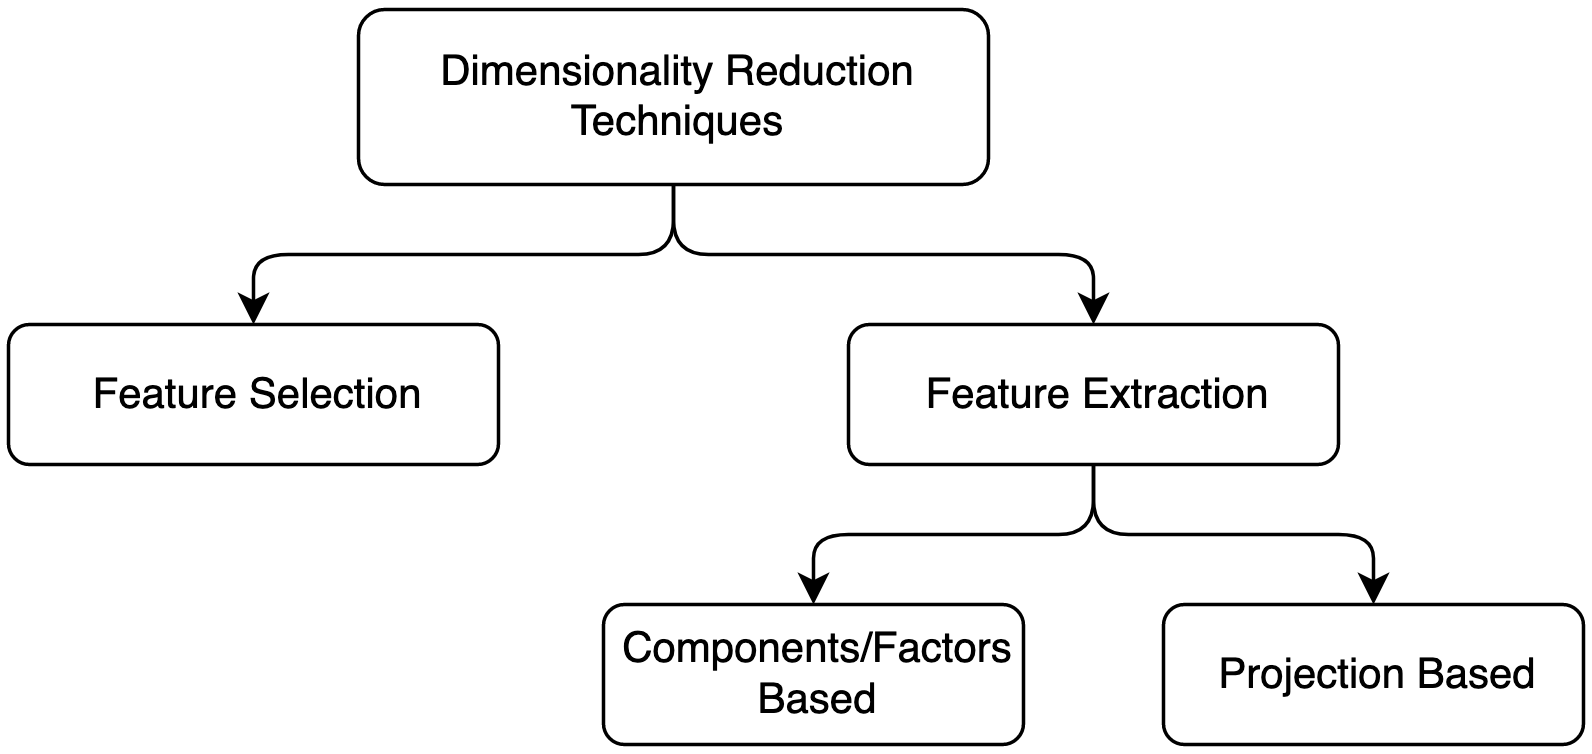
\includegraphics[width=1\linewidth]{dimensionality_reduction.png}
  \caption{Dimensionality Reduction Techniques}
  \label{fig:dimensionality-reduction}
\end{figure}

Although all these methods reduce the dimensionality of data, the means used to
do so varies.

\subsection*{Feature Selection}

Feature selection methods reduce dimensionality through the selection of the
most important features among the ones already existing in the dataset. The
criterion used either improves, maintains the model accuracy, or simplifies the
model complexity. Below are presented commonly used supervise feature selection
methods. For more information on listed and/or additional methods the reader is
directed to \cite{Cai2018, Ghojogh2019}.

\begin{enumerate}
  % TODO: find references
  \item Correlation based feature selection (CFS). It's based on the predictive
  power of a feature subset, found by computing the correlation between the
  feature subset and the target feature. It is therefore a generalisation
  of the Correlation Criteria as defined in \cite{Ghojogh2019}.
  \item ReliefF \cite{kononenko1997}. It's an extension of Relief
  \cite{kira1992} to support multi-class problems. For each instance, the
  algorithm considers the closest instance from each class to update the
  feature score vector. The score of any given feature decreases if it differs
  more in nearby instances of the same class than nearby instances of the other
  class, and increases in the reverse case.
  % TODO: Find references
  \item Random Subspace Method (RSM) and Random Forest Method (RFM). Consists
  in the training of base classifiers on different feature subsets. These
  methods use the trained classifiers to assess each feature's importance to
  the prediction of the target variable. In the case of RFM, it is important to
  consider that Tree based classifiers are trained through the minimisation of
  entropy on each data split. As such, variables used earlier for decision
  rules along a decision tree's path is deemed as having a higher importance
  than the remaining variables.
\end{enumerate}

% TODO: Find references
Along with the presented methods, a number of variations are being applied by
practitioners, such as Permutation Feature Importance (shuffling each feature
after training a classifier and check accuracy drops) and Drop Column Feature
Importance (dropping one feature and checking differences in accuracy compared
to a classifier using all available features).


\subsection*{Feature Extraction}
TODO


\section{Data Filtering Methods}

The accuracy of a classifier is directly affected by the quality the training
data used \cite{Boukir2019}. Although classification is an important task in
remote sensing, obtaining well-labelled data is time consuming, impracticable
and expensive \cite{Pelletier2017Filtering}. Although no systematic review on
data selection/filtering methods for the remote sensing domain was found, 2
distinct types of filtering were identified.

LULC maps are commonly presented in a shapefile format. A recent study
employed polygon membership information for each pixel to detect labelling
errors within each polygon. This was done through the use of clustering methods
and cross cluster consistency measurement methods \cite{Paris2019}. Variations
on this method are explored and documented below.

A frequent type of approach to address this challenge is based on the use of
different machine learning classifiers to detect these errors
\cite{Brodley1999, Jiang2004, Liu2008, Yuan2018, Zhang2018,
Pelletier2017Filtering, Garcia-Gil2019, Boukir2019, Zhang2019}. These methods
benefit from classifiers' specificities, especially Random Forest, to implement
different voting strategies and model fitting methods to improve label noise
detection. Since these methods don't use domain specific information, they can
be used over any machine learning problem.

Although the impact of these filtering methods on robust classifiers is
unknown, some studies document the impact of label noise on classification
accuracy, showing the robustness of Random Forests and Deep Learning algorithms
\cite{Pelletier2017Effect, Rolnick2017}. Relevant filtering methods presented
in this section will incorporate the experiment, where the impact of data
filtering can be assessed (although these results are accompanied with
significant limitations).

% In order to add an unnumbered section/chapter:
%\addcontentsline{toc}{section}{Uppgift 1}
\subsection*{Cluster-based methods}

The best performing label noise detection algorithm based on clustering methods was proposed by \cite{Paris2019}. This method assumes the availability of a LULC map provided at a polygon level. The training set identification method is based on 3 steps: 1) Polygon k-means clustering, 2) Polygon consistency analysis and 3) Stratified Random Sampling

\subsubsection{Variations on cluster-based methods}
TODO

\subsection*{Classifier-based methods}
TODO

\subsubsection{Variations on classifier-based methods}
TODO

\section{Classification Methods}
TODO

\chapter{Methodology}

\section{Datasets}

\section{Preprocessing}

\section{Data Filtering}

\section{Classification}

\chapter{Results and Discussion}



% Adding a bibliography if citations are used in the report
\bibliographystyle{plain}
\bibliography{references.bib}
% Adds reference to the Bibliography in the ToC
\addcontentsline{toc}{chapter}{\bibname}


\end{document}
